\chapter{Weitere FEM-Ergebnisse}\label{sec:mehrFEM}


\begin{figure}[h]
	\begin{minipage}[t]{0.5\linewidth}
		\centering
		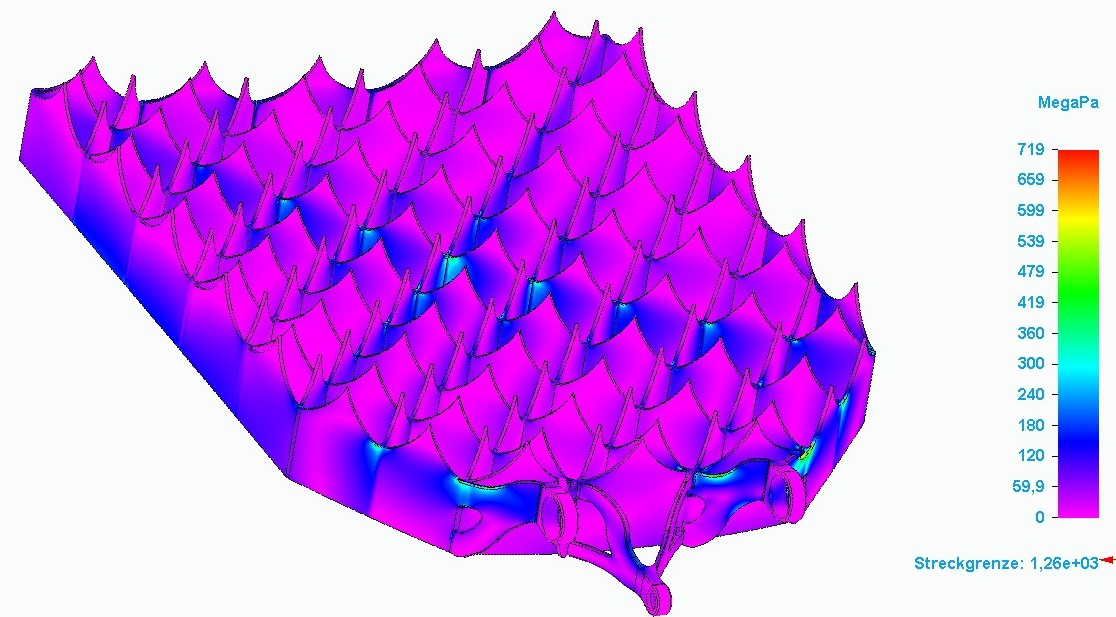
\includegraphics[width=0.95\textwidth]{D1 3.9 t.jpg}
		\caption{Tal-Typus D1}
	\end{minipage}
	\hfill
	\begin{minipage}[t]{0.5\linewidth}
		\centering
		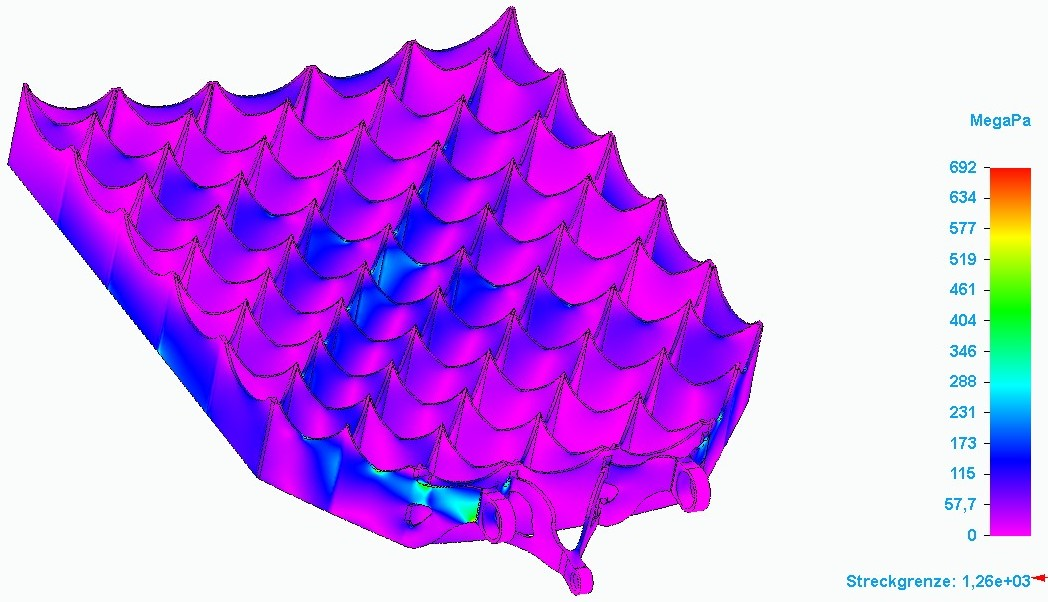
\includegraphics[width=0.95\textwidth]{D1 3.9 b.jpg}
		\caption{Berg-Typus D1}
	\end{minipage}
\end{figure}
\begin{figure}[h]
\begin{minipage}[t]{0.5\linewidth}
	\centering
	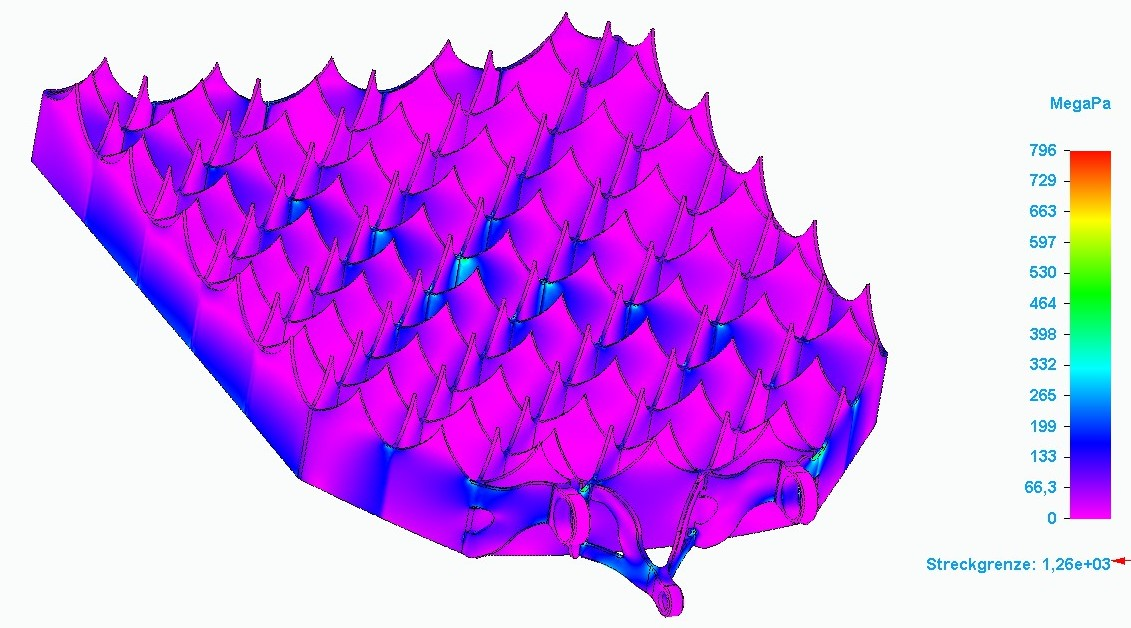
\includegraphics[width=0.95\textwidth]{D2 3.9 t.jpg}
	\caption{Tal-Typus D2}
\end{minipage}
\hfill
\begin{minipage}[t]{0.5\linewidth}
	\centering
	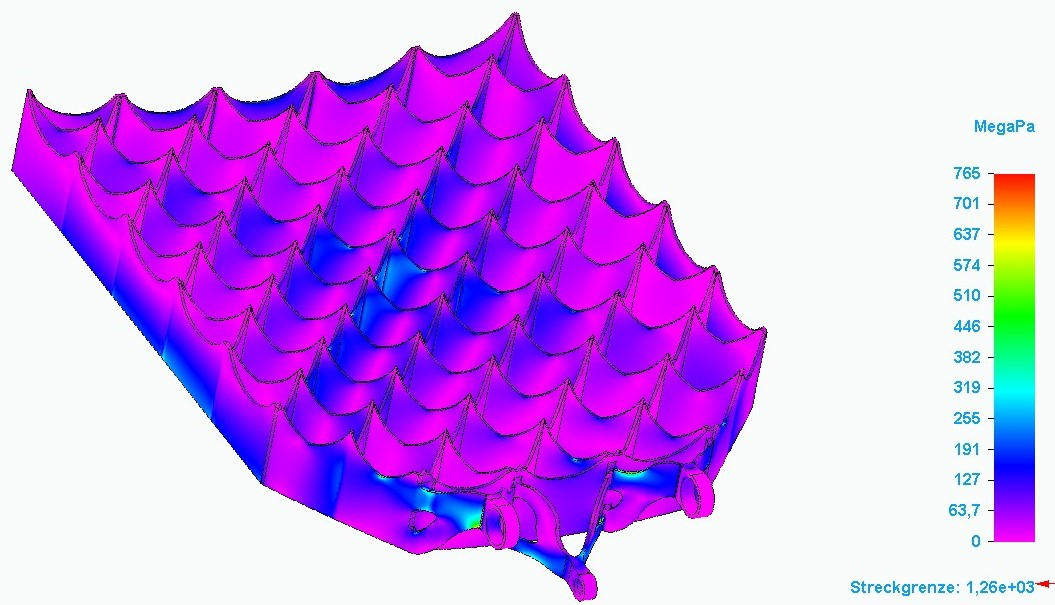
\includegraphics[width=0.95\textwidth]{D2 3.9 b.jpg}
	\caption{Berg-Typus D2}
\end{minipage}
\end{figure}
\begin{figure}[h]
\begin{minipage}[t]{0.5\linewidth}
	\centering
	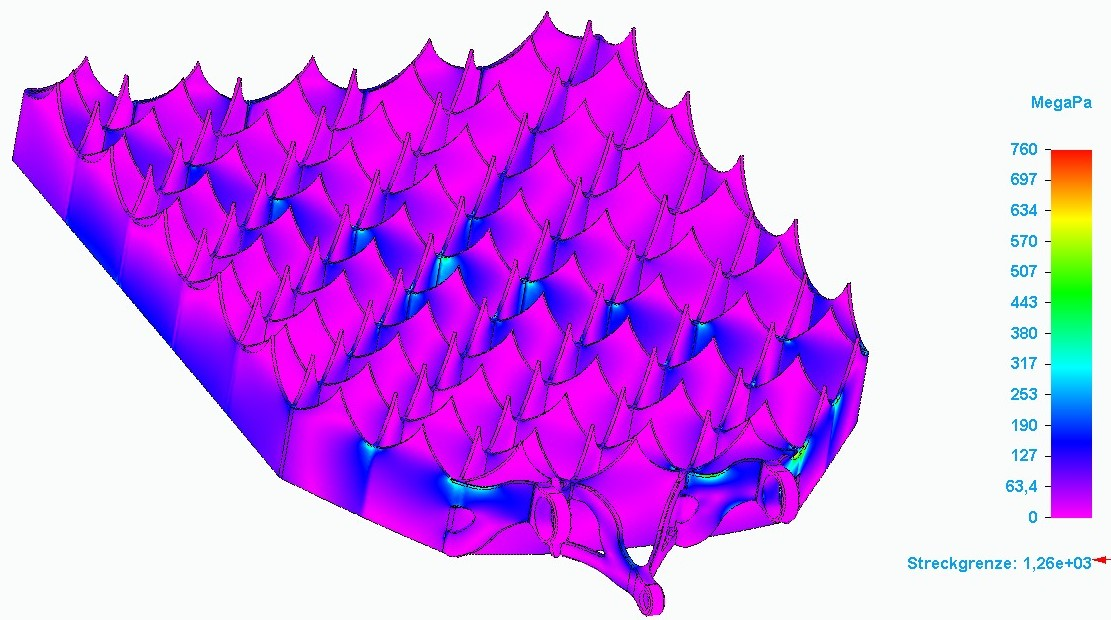
\includegraphics[width=0.95\textwidth]{R1 3.9 t.jpg}
	\caption{Tal-Typus R1}
\end{minipage}
\hfill
\begin{minipage}[t]{0.5\linewidth}
	\centering
	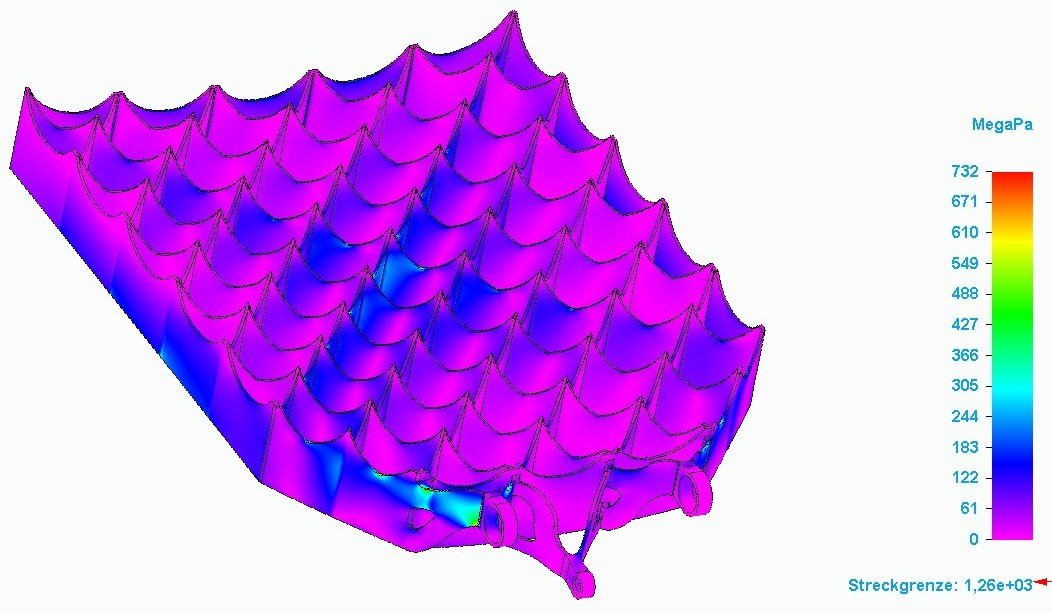
\includegraphics[width=0.95\textwidth]{R1 3.9 b.jpg}
	\caption{Berg-Typus R1}
\end{minipage}
\end{figure}
%
%
\begin{figure}[h]
\begin{minipage}[t]{0.5\linewidth}
	\centering
	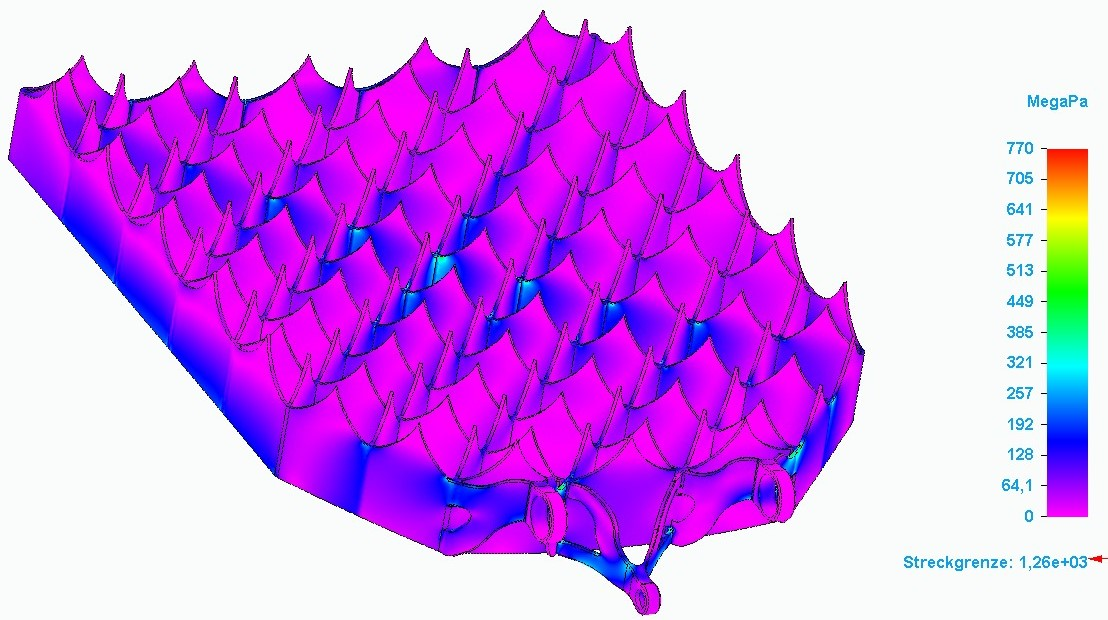
\includegraphics[width=0.95\textwidth]{R2 3.9 t.jpg}
	\caption{Tal-Typus R2}
\end{minipage}
\hfill
\begin{minipage}[t]{0.5\linewidth}
	\centering
	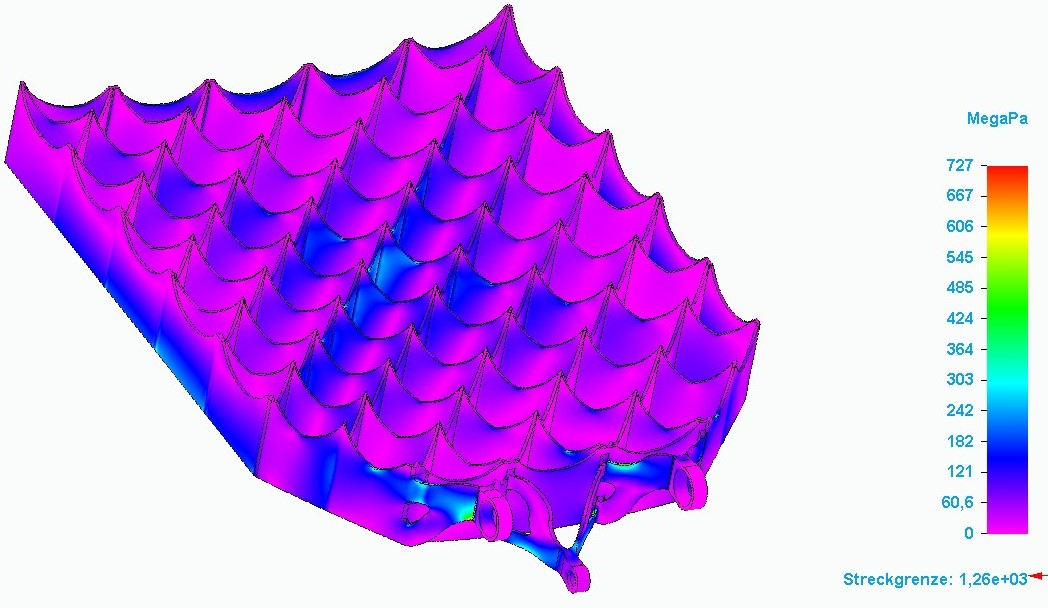
\includegraphics[width=0.95\textwidth]{R2 3.9 b.jpg}
	\caption{Berg-Typus R2}
\end{minipage}
\end{figure}
\begin{figure}[h]
\begin{minipage}[t]{0.5\linewidth}
	\centering
	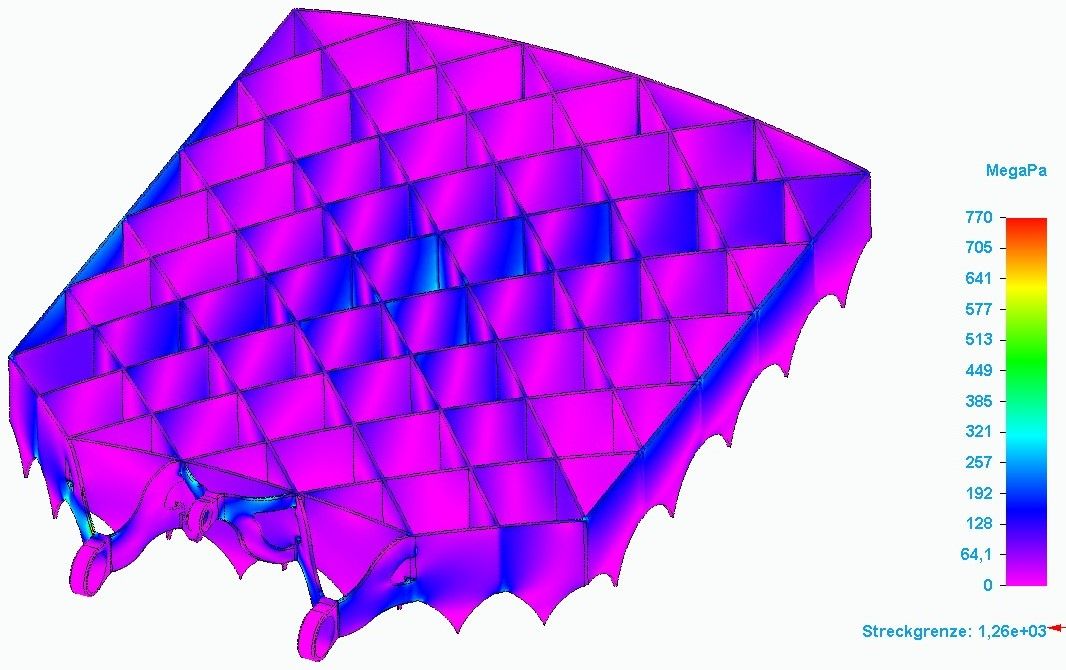
\includegraphics[width=0.95\textwidth]{20g 3.9 t.jpg}
	\caption{Tal-Typus beim maximalen Lastenvielfachen}
\end{minipage}
\hfill
\begin{minipage}[t]{0.5\linewidth}
	\centering
	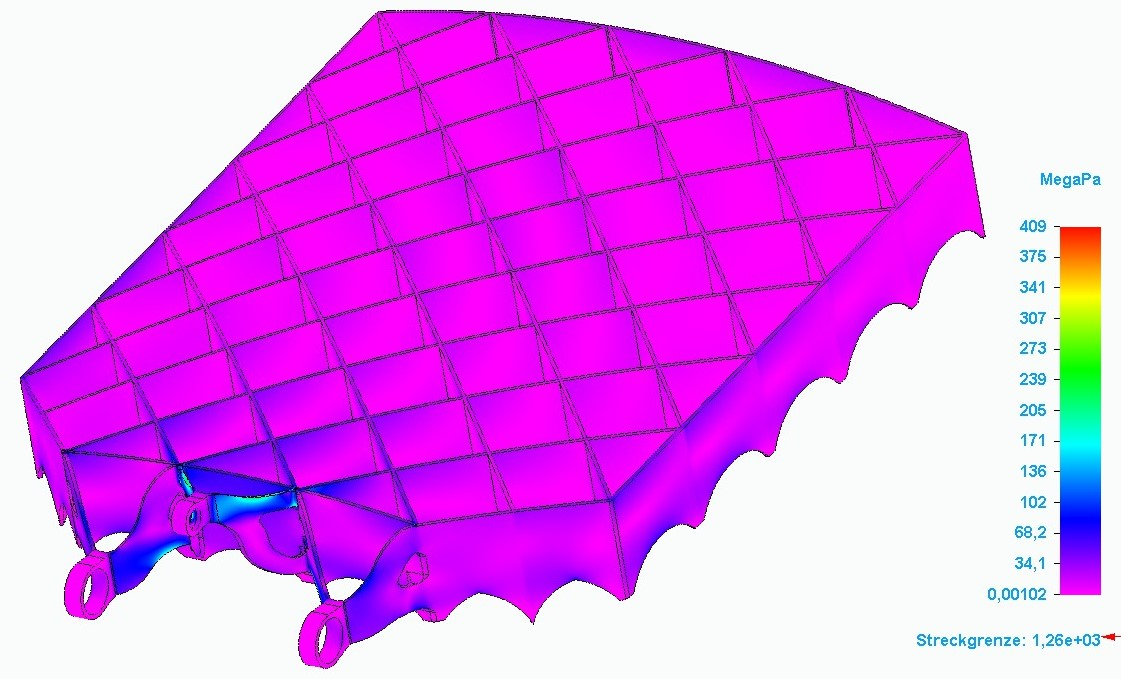
\includegraphics[width=0.95\textwidth]{20g 3.9 b.jpg}
	\caption{Berg-Typus beim maximalen Lastenvielfachen}
\end{minipage}
\end{figure}